\subsection{Krzyżowanie}

\subsubsection{Kod źródłowy}



\subsubsection{Wyniki badań}

\begin{figure}[H]
	\centering
	\hspace*{-0.8in}
	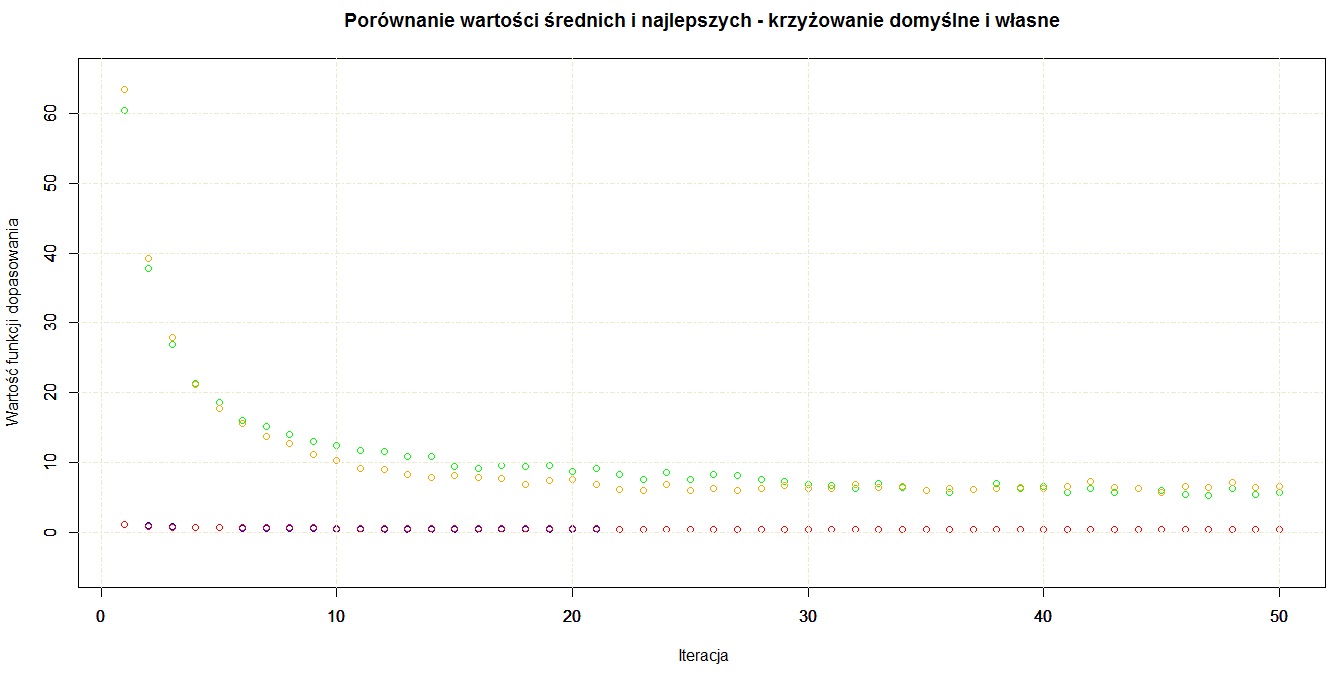
\includegraphics[scale = 0.5]{cross_0_2}
	\caption{Wykres dla prawdopodobieństwa krzyżowania 0.2}  
	\label{rys:cross_0_2} 
\end{figure}


\begin{figure}[H]
	\centering
	\hspace*{-0.8in}
	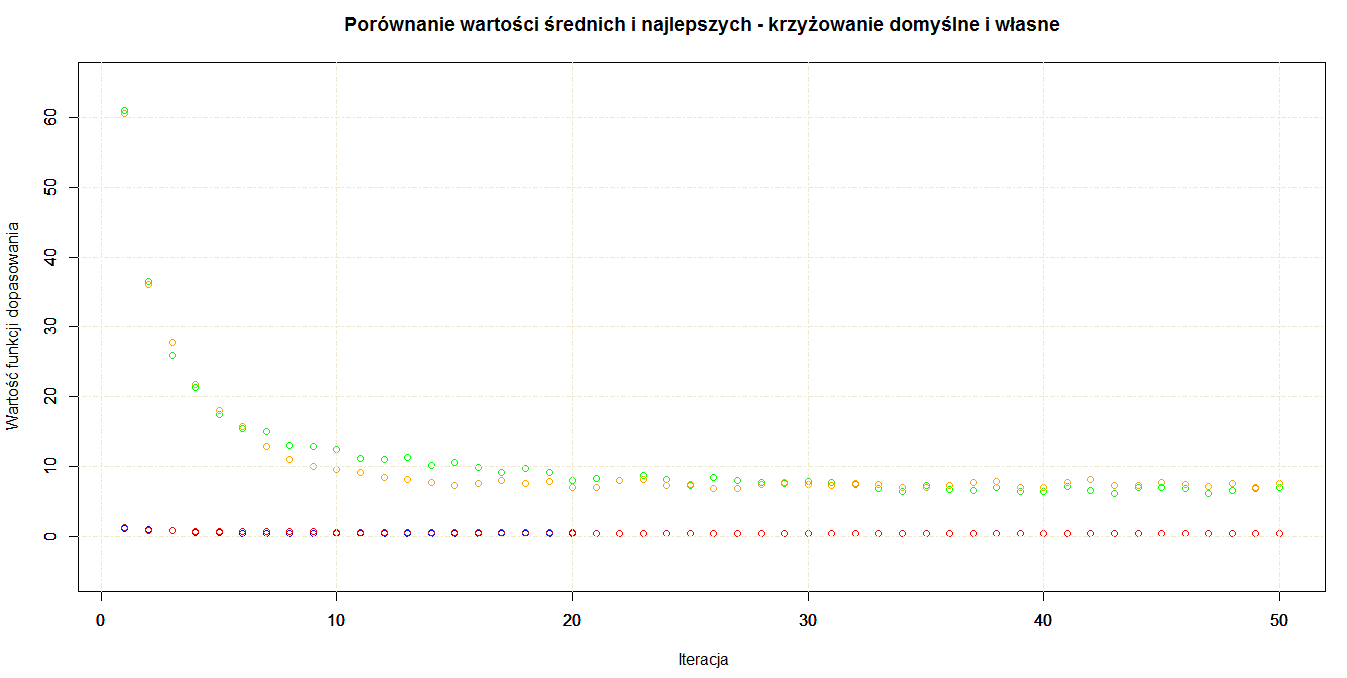
\includegraphics[scale = 0.5]{cross_0_5}
	\caption{Wykres dla prawdopodobieństwa krzyżowania 0.5}  
	\label{rys:cross_0_5} 
\end{figure}


\begin{figure}[H]
	\centering
	\hspace*{-0.8in}
	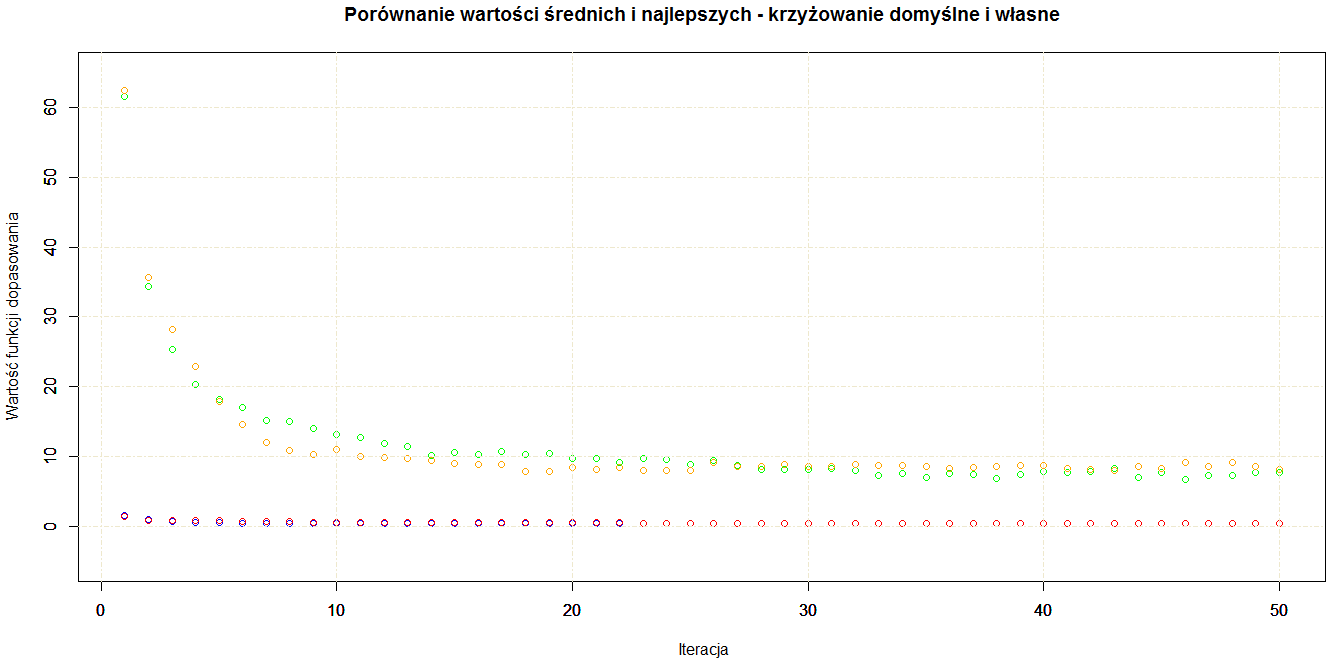
\includegraphics[scale = 0.5]{cross_0_7}
	\caption{Wykres dla prawdopodobieństwa krzyżowania 0.7}  
	\label{rys:cross_0_7} 
\end{figure}


\begin{figure}[H]
	\centering
	\hspace*{-0.8in}
	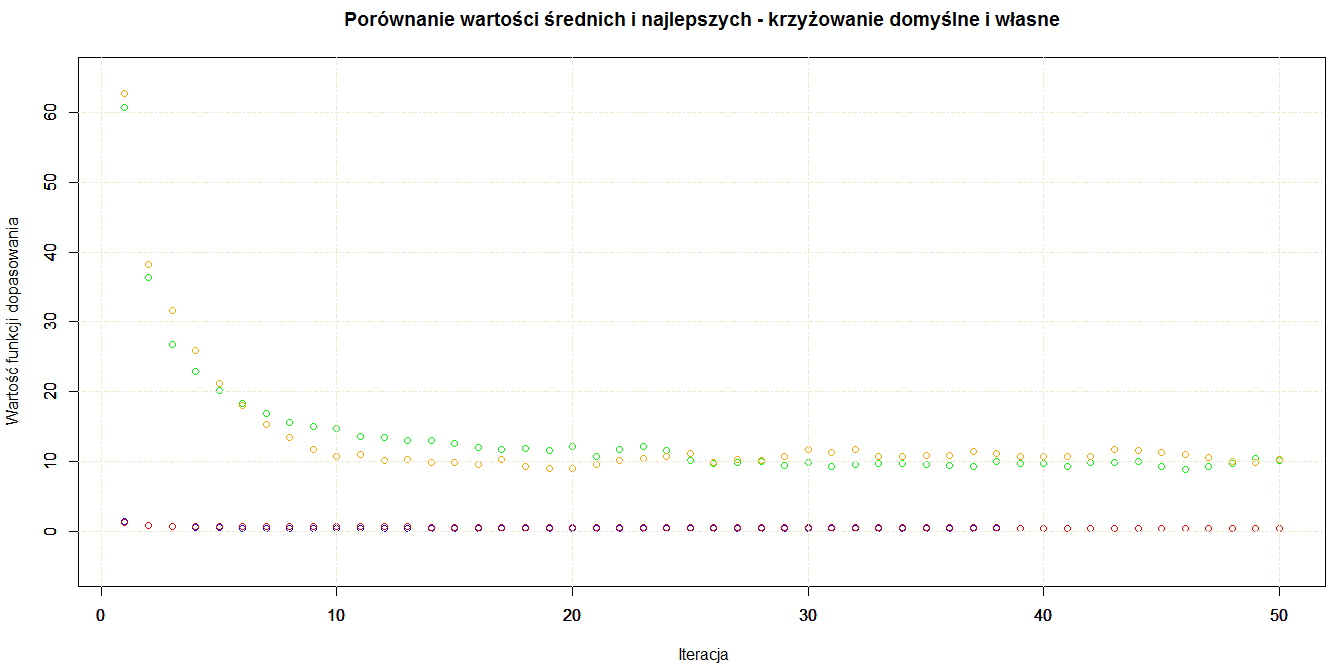
\includegraphics[scale = 0.5]{cross_1}
	\caption{Wykres dla prawdopodobieństwa krzyżowania 1}  
	\label{rys:cross_1} 
\end{figure}


\subsubsection{Wnioski}

\begin{table}[!h]
	\centering
	\caption{Wartości średnie i najlepsze osobnika dla domyślnej i własnej funkcji krzyżowania}
	\label{cross_porownanie}
	\hspace*{-0.5in}
	\begin{tabular}{|c|c|c|c|c|}
		\hline
		\textbf{Prawdopodobieństwo} & \multicolumn{2}{c}{\textbf{Krzyżowanie domyśln}}  & \multicolumn{2}{|c|}{\textbf{Krzyżowanie własne}} \\ \cline{2-5}
		\textbf{krzyżowania} & Wartość średnia & Najlepszy wynik & Wartość średnia & Najlepszy wynik \\ \hline
		
		0.2 & 5.697605 & 0.399347 & 6.538159 & 0.440933 \\
		0.5 & 6.973119 & 0.398064 & 7.590295 & 0.457468 \\
		0.7 & 7.753576 & 0.398096 & 8.148286 & 0.464140 \\
		1   & 10.206810 & 0.398485 & 10.375570 & 0.476180  \\ \hline      
	\end{tabular}
\end{table}